\section{Generation Mechanisms}\label{sec:generation-mechanisms}

In this section, we provide a general description of the synthetic data
generation mechanisms found in the learning problems in
Section~\ref{sec:algorithmic-applications}.
Table~\ref{tbl:generation-mechanisms} summarizes the assumptions and usage of
the generation mechanisms across the selected works and learning problems.

\begingroup\small
\begin{longtable}{clcccccccc}
    \caption{Analysis of synthetic data generation mechanisms.}
    \label{tbl:generation-mechanisms}\\
    \toprule
        Type & Mechanism & Smoothness & Manifold & Priv. & Reg. & Ovs. & AL & Semi-SL & Self-SL \\
    \midrule
    \endfirsthead
    \caption[]{Analysis of synthetic data generation mechanisms.} \\
    \toprule
        Type & Mechanism & Smoothness & Manifold & Priv. & Reg. & Ovs. & AL & Semi-SL & Self-SL \\
    \midrule
    \endhead
    \midrule
    \multicolumn{9}{r}{{Continued on next page}} \\
    \midrule
    \endfoot
    
    \bottomrule
    \endlastfoot
    \multirow{5}{*}{Perturbation} 
        & Random         & \checkmark & \checkmark 
                         & $\times$ & $\times$ & \checkmark & $\times$ & $\times$ & $\times$ \\

        & Laplace        & \checkmark & \checkmark 
                         & \checkmark & $\times$ & $\times$ & $\times$ & $\times$ & $\times$ \\

        & Gaussian       & \checkmark & \checkmark 
                         & \checkmark & \checkmark & $\times$ & $\times$ & \checkmark & \checkmark \\

        & Swap-noise     & $\times$ & $\times$ 
                         & $\times$ & $\times$ & $\times$ & $\times$ & \checkmark & \checkmark \\

        & Zero-out noise & $\times$ & $\times$ 
                         & $\times$ & $\times$ & $\times$ & $\times$ & $\times$ & \checkmark \\

    \midrule
    \multirow{3}{*}{PDF} 
        & Gaussian Gen. & $\times$ & \checkmark 
                        & \checkmark & $\times$ & \checkmark & $\times$ & $\times$ & $\times$ \\

        & Gaussian Mix. & $\times$ & \checkmark 
                        & \checkmark & $\times$ & \checkmark & $\times$ & $\times$ & $\times$ \\

        & KDE           & $\times$ & \checkmark 
                        & $\times$ & $\times$ & \checkmark & $\times$ & $\times$ & $\times$ \\

    \midrule
    \multirow{3}{*}{PGM} 
        & Bayesian Net. & $\times$ & $\times$ 
                        & \checkmark & \checkmark & $\times$ & $\times$ & $\times$ & $\times$ \\

        & Gibbs         & $\times$ & $\times$ 
                        & $\times$ & \checkmark & \checkmark & $\times$ & $\times$ & $\times$ \\

        & Random Walk & $\times$ & $\times$
                      & $\times$ & $\times$ & \checkmark & $\times$ & $\times$ & $\times$ \\


    \midrule
    \multirow{6}{*}{Linear} 
        & Between-class Int.  & $\times$ & \checkmark   
                              & $\times$ & \checkmark & $\times$ & \checkmark & \checkmark & $\times$ \\

        & Within-class Int.   & \checkmark & \checkmark 
                              & $\times$ & \checkmark & \checkmark & \checkmark & \checkmark & $\times$ \\
        
        & Extrapolation       & \checkmark & \checkmark 
                              & $\times$ & \checkmark & \checkmark & $\times$ & $\times$ & $\times$ \\

        & Hard Extra.         & \checkmark & \checkmark 
                              & $\times$ & \checkmark & \checkmark & $\times$ & $\times$ & $\times$ \\

        & Inter.+Extra.       & \checkmark & \checkmark 
                              & $\times$ & $\times$ & \checkmark & $\times$ & $\times$ & $\times$ \\

        & Difference Transf.  & \checkmark & \checkmark 
                              & $\times$ & \checkmark & $\times$ & $\times$ & $\times$ & $\times$ \\


    \midrule
    \multirow{3}{*}{Geometric} 
        & Hypersphere & \checkmark & \checkmark 
                      & $\times$ & $\times$ & \checkmark & \checkmark & $\times$ & $\times$ \\

        & Triangular  & \checkmark & \checkmark
                      & $\times$ & $\times$ & $\times$ & $\times$ & \checkmark & $\times$ \\

        & Hyperrectangle & $\times$ & \checkmark 
                         & $\times$ & \checkmark & $\times$ & $\times$ & $\times$ & $\times$ \\
    \midrule
    \multirow{2}{*}{Neural nets.} 
        & GAN & $\times$ & $\times$ 
              & \checkmark & \checkmark & \checkmark & \checkmark & $\times$ & $\times$ \\

        & AE & $\times$ & $\times$ 
             & $\times$ & \checkmark & \checkmark & \checkmark & \checkmark & $\times$ \\
    \midrule
    \multirow{2}{*}{Others}
        & Exponential M. & $\times$ & $\times$
                         & \checkmark & $\times$ & $\times$ & $\times$ & $\times$ & $\times$ \\

        & Reconstruction err. & $\times$ & $\times$ 
                               & $\times$ & $\times$ & \checkmark & $\times$ & $\times$ & $\times$ \\
\end{longtable}
\endgroup


We focus on 2 key conditions for the data generation process, smoothness, and
manifold space (adapted from the background in~\cite{Van2020}). The
smoothness condition requires that if two observations $x_i, x_j$ are close,
then it's expected that $y_i, y_j$ have the same value.  The manifold
condition requires synthetic data generation to occur within local Euclidean
topological spaces. Therefore, a generation mechanism with the smoothness
requirement also requires a manifold, while the opposite is not necessarily
true.

In the remaining subsections, we will describe the main synthetic data
generation mechanisms found in the literature, based on the studies discussed
in Section~\ref{sec:algorithmic-applications}.

\subsection{Perturbation Mechanisms}

The general perturbation-based synthetic data generation mechanism is defined
as $x^s = x_i + \epsilon$, where $\epsilon$ is the noise vector sampled from a
certain distribution. The random perturbation mechanism can be thought of as
the non-informed equivalent of PGMs and PDFs. It samples $|\epsilon|$ values
from a uniform distribution, \textit{i.e.}, $e_i \sim \mathcal{U}(\cdot,
\cdot), \forall e_i \in \epsilon$, while the minimum and maximum values depend
on the context and level of perturbation desired, typically centered around
zero.

Laplace (commonly used in DP algorithms) and Gaussian perturbations sample
$\epsilon$ with $e_i \sim \text{Lap}(\cdot, \cdot)$ and $e_i \sim
\mathcal{N}(\cdot, \cdot)$, respectively. Within the applications found, in
the presence of categorical features, these methods tend to use n-way
marginals (also known as conjunctions or contingency
tables~\cite{gaboardi2014dual}) to ensure the generated data contains
variability in the categorical features and the distribution of categorical
feature values follows some given constraint. Although various other
distributions could be used to apply perturbations, the literature found
primarily focuses on introducing noise via uniform, Laplace, and Gaussian
distributions.

\begin{figure}
	\centering
	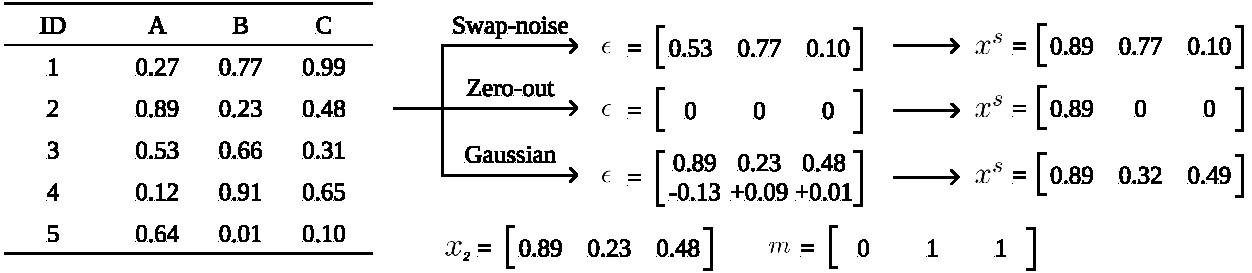
\includegraphics[width=.95\linewidth]{figures/synthetic-data-review/masking-example}
    \caption{Examples of synthetic observations generated with different
        masking approaches.
    }~\label{fig:masking-example}
\end{figure}

Masking modifies the original perturbation-based approach by introducing a
binomial mask vector, $m = [m_1, \ldots, m_d]^\bot \in \{0,1\}^d, m_i \sim
\text{Bern}(p_m)$ and the generation mechanism is defined as $x^s = (1 -
m)\odot x_i + m \odot \epsilon$~\cite{yoon2020vime}. The $\epsilon$ variable
is defined according to the perturbation used. The Gaussian approach generates
the noise vector as $\epsilon = x_i + \epsilon'$, where $e_i' \sim
\mathcal{N}(\cdot, \cdot), \forall e_i' \in \epsilon'$. The swap-noise
approach shuffles the feature values from all observations to form
$\epsilon$, while the zero-out noise approach sets all $\epsilon$ values to
zero. Intuitively, the masking technique modifies an observation's feature
values with probability $p_m$, instead of adding perturbations over the
entire observation. Figure~\ref{fig:masking-example} shows a visual depiction
of the masking technique.

\subsection{Probability Density Function Mechanisms}

The Gaussian generative model, despite being infrequently used when compared to the
remaining Probability Density Function mechanisms discussed in this subsection,
is an essential building block for these mechanisms. In particular, we focus
on the multivariate Gaussian approach, which follows near-Gaussian
distribution assumptions, which is rarely reasonable on the input space.
However, for high-dimensional data, it is possible to motivate this approach
via the \textit{Diaconis-Freedman-Meckes} effect~\cite{meckes2012projections},
which states that high-dimensional data projections generally follow a nearly
Gaussian distribution. The Gaussian generative model produces synthetic data
from a Gaussian distribution $x^s \sim \mathcal{N}(\mu, \Sigma)$, where $\mu
\in \mathbb{R}^d$ is a vector with the features' means and $\Sigma \in
\mathbb{R}^{d \times d}$ is the covariance matrix. It follows the following
density function~\cite{chanyaswad2019ron}:

\begin{equation}\label{eq:gaussian}
    f(x) =
    \frac{1}{\sqrt{(2\pi)^d\text{det}(\Sigma)}}\text{exp}\left(-\frac{1}{2}(x-\mu)^T\Sigma^{-1}(x-\mu)\right)
\end{equation}

Consequently, to define a Gaussian generative model it is only necessary to
estimate the dataset's mean and covariance matrix.

A Gaussian mixture model (GMM) comprises several Gaussian distributions that
aim to represent subpopulations within a dataset. Its training procedure
allows the model to iteratively learn the subpopulations using the Expectation
Maximization algorithm. A GMM becomes more appropriate than the Gaussian
generative model when the data is expected to have more than one
higher-density region, leading to a poor fit of unimodal Gaussian models.

Kernel Density Estimation (KDE) methods use a kernel function to estimate the
density of the dataset's distribution at each region of the input/latent
space. Despite the various kernel options, the Gaussian kernel is commonly
used for synthetic data generation~\cite{tang2015kerneladasyn}. The general
kernel estimator is defined as follows: 

\begin{equation}
    \hat{p}(x) = \frac{1}{N+h}
    \sum_{i=1}^{N}K\left(\frac{x-x_i}{h}\right)
\end{equation}

Where $N = |\mathcal{D}|$, $h$ is a smoothing parameter known as bandwidth and
$K$ is the kernel function. The Gaussian kernel is defined as follows:

\begin{equation}
    G_i(x) = K\left(\frac{x-x_i}{h} \right) = \frac{1}{(\sqrt{2\pi} h)^d} 
    \text{exp}\left(-\frac{1}{2}\frac{(x-x_i)^T(x-x_i)}{h}\right) 
\end{equation}

Therefore, the Gaussian KDE approach can also be expressed as $\hat{p}(x) =
\frac{1}{N+h}\sum_{i=1}^{N}G_i(x)$, while the data is sampled from the
estimated probability distribution. Figure~\ref{fig:pdf-example} shows a
visualization of the PDF mechanisms discussed, applied to a mock dataset.

\begin{figure}
	\centering
	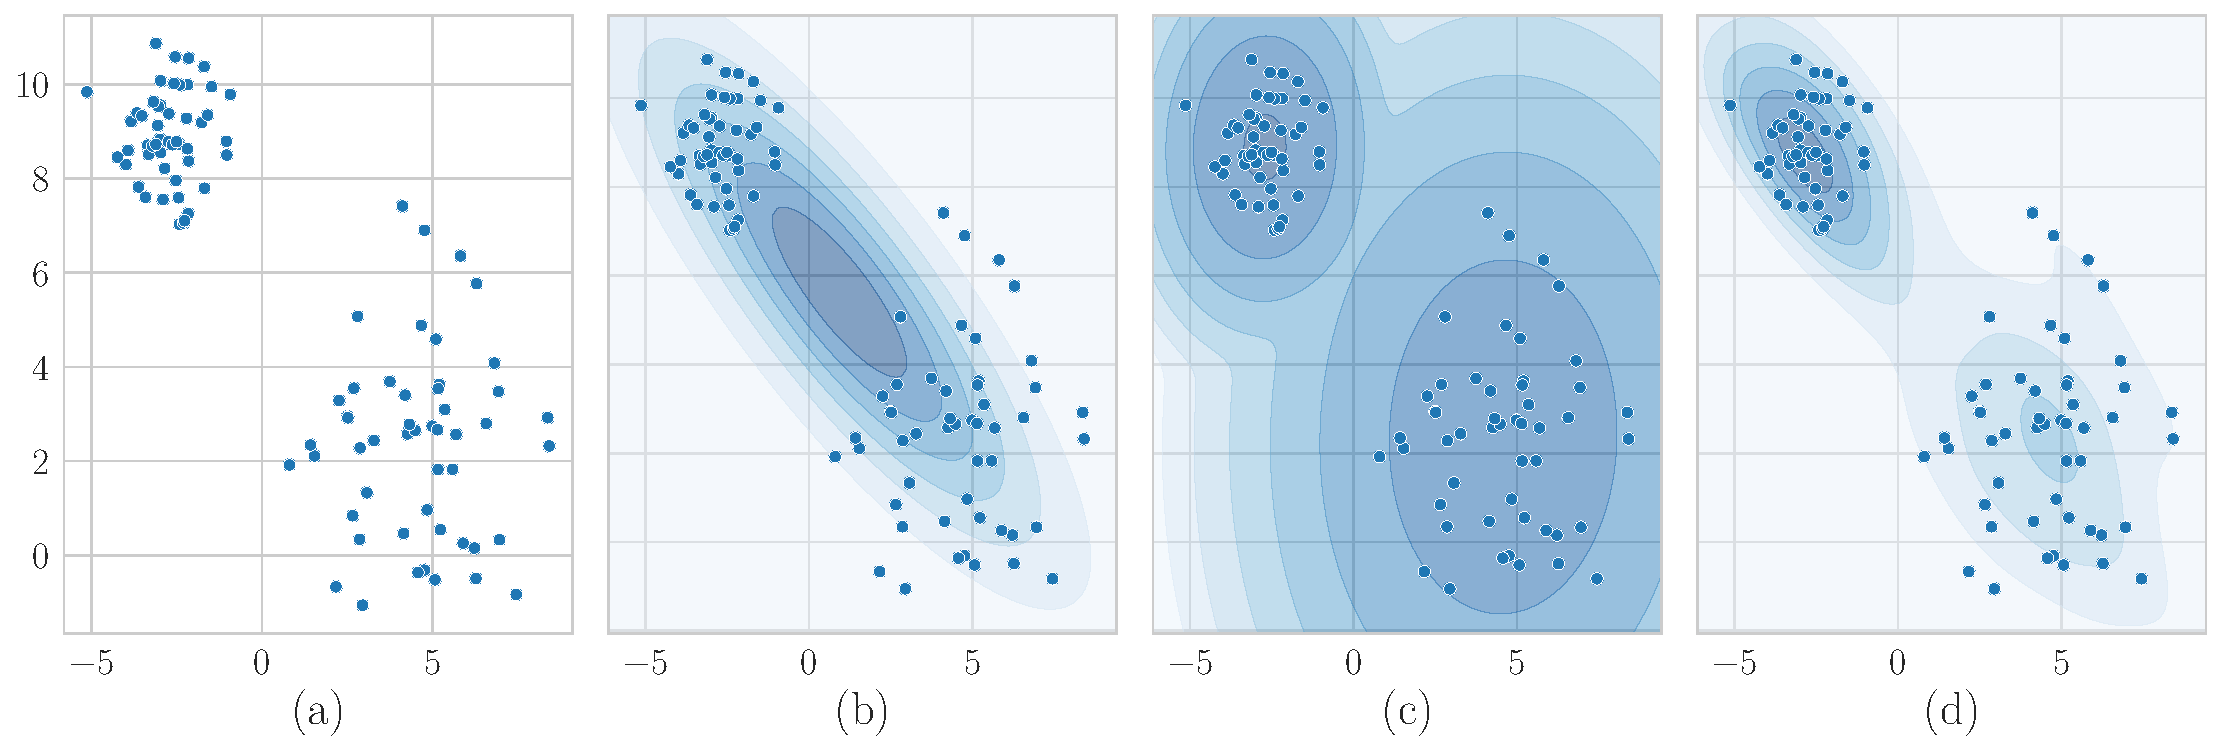
\includegraphics[width=.95\linewidth]{figures/synthetic-data-review/pdf-example}
    \caption[Examples of PDF mechanisms fitted to a mock dataset.]{%
        Examples of PDF mechanisms fitted to a mock dataset. Legend: (a)
        Original dataset, (b) Gaussian generative model, (c) Gaussian Mixture
        Model and (d) Gaussian Kernel Density Estimation.
    }~\label{fig:pdf-example}
\end{figure}

\subsection{Probabilistic Graphical Models}

A Bayesian network can be thought of as a collection of
conditional distributions. It represents the joint probability distribution
over the cross-product of the feature domains in $\mathcal{D}$. It is a
directed acyclic graph that represents $\mathcal{D}$'s features as nodes and
their conditional dependencies as directed edges. The set of features pointing
directly to feature $v \in V, d=|V|$ via a single edge are known as the parent
variables, $pa(v)$. A Bayesian network calculates $p(x)$ as the product of the
individual density functions, based on the conditional probabilities of the
parent variables:

\begin{equation}
    p(x) = \prod_{v \in V} p(x_v | x_{pa(v)})
\end{equation}

Since the construction of a directed acyclic graph can be labor intensive,
different ML approaches were developed for the learning of these
structures~\cite{yu2019dag}. Bayesian networks can be used for synthetic data
generation when the relationship between variables is known (or can be
learned) and when the data is high-dimensional, making the sampling process
non-trivial.

Random walk algorithms comprise the general process of iterating through a set
of random steps. Although uncommon, random walk approaches may be used to
sample data. The random walk approach described in \cite{zhang2014rwo} uses
the Gaussian noise mechanism over minority class observations to create
synthetic observations. The Gibbs sampling mechanism also performs a random
walk by iterating through sampled feature values.

Gibbs sampling is a Markov Chain Monte Carlo algorithm that iteratively
samples a synthetic observation's feature values. It is a suitable method to
sample synthetic data from a Bayesian network. The process starts with an
initial observation selected from $\mathcal{D}$, $x_0$, and is used to begin
the sampling process. In its original format, the sampling of each feature
value $v$ in $x^s_i$ is conditioned by $x^s_{i-1}$ and the feature values
already sampled from $x^s_i$, such that $x^s_{i, v} \sim p(x^s_{i, v} |
x^s_{i, 1}, \ldots, x^s_{i, v-1}, x^s_{i-1, v+1}, \dots, x^s_{i-1, d})$.
Therefore, Gibbs sampling is a special case of the Metropolis-Hastings
algorithm.

\subsection{Linear Transformations}

Linear interpolation mechanisms can be split into two subgroups: between and
within-class interpolation. Both mechanisms follow a similar approach; they
use a scaling factor $\lambda$, typically sampled from either
$\mathcal{U}(0,1)$ or $\text{Beta}(\alpha, \alpha)$: 

\begin{equation}~\label{eq:interpolation}
    x^s = \lambda x_i + (1-\lambda)x_j = x_j + \lambda(x_i - x_j)
\end{equation}

The within-class interpolation mechanism selects two observations from the
same class, while the between-class interpolation mechanism selects two
observations from different classes and also interpolates the one-hot encoded
target classes $y_i$ and $y_j$. However, the approach to select observations
might vary according to the ML task and data generation algorithm. For
example, most SMOTE-based methods select a center observation and a random
observation within its $k$-nearest neighbors belonging to the same class,
while the Mixup method selects two random observations, regardless of their
class membership.

\begin{figure}
	\centering
	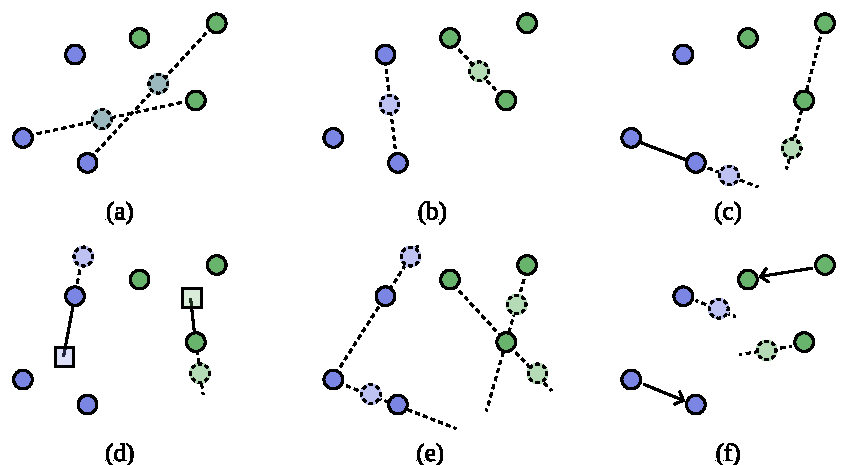
\includegraphics[width=.7\linewidth]{figures/synthetic-data-review/linear-transformations}
    \caption[Examples of linear transformation mechanisms.]{%
        Examples of linear transformation mechanisms. Legend: (a)
        Between-class interpolation, (b) Within-class interpolation, (c)
        Observation-based extrapolation, (d) Hard extrapolation, (e)
        Combination of interpolation and extrapolation and (f) Difference
        transform.
    }~\label{fig:linear-transformations}
\end{figure}

The observation-based linear extrapolation mechanism modifies
Equation~\ref{eq:interpolation} such that $x^s = x_i + \lambda(x_i - x_j)$,
while the hard extrapolation mechanism uses the mean of a class' observations,
$\mu^c$ and a randomly selected observation to generate $x^s = x_i^c +
\lambda(x_i^c - \mu^c)$. Some methods also combine both interpolation and
extrapolation. This can be achieved using Equation~\ref{eq:interpolation} and
modifying $\lambda$'s range to either decrease its minimum value below zero
or increase its maximum value above one.

The difference transform mechanism uses two observations to compute a
translation vector (multiplied by the scaling factor $\lambda$) and apply it
to a third observation:

\begin{equation}
    x^s = x_i + \lambda(x_j - x_k)
\end{equation}

Although there are various linear transformation mechanisms in the literature,
the majority of the studies applied linear interpolation mechanisms.
Within-class interpolation was frequently found in oversampling methods, while
between-class interpolation was found most often in regularization methods. A
depiction of the linear transformation mechanisms found in the literature
is presented in Figure~\ref{fig:linear-transformations}.

\subsection{Geometric Transformations}

Overall, geometric transformation mechanisms were not frequently found in the
literature. They are primarily used to develop Mixup or SMOTE-based variants.
Figure~\ref{fig:geometric-transformations} shows a visual example of the
related mechanisms.

The hypersphere mechanism generates data within a distorted, n-dimensional
hyper spheroid. It is formed using an observation to define the center of
the geometry and another to define its edge.
It is defined with two hyperparameters, the deformation
factor, $\alpha_{def} \in [0, 1]$, and the truncation factor, $\alpha_{trunc}
\in [-1, 1]$. The deformation factor deforms the hypersphere into an elliptic
shape, where $\alpha_{def}=1$ applies no deformation and $\alpha_{def}=0$
creates a line segment. The truncation factor limits the generation area of
the hyper spheroid within a subset of the hypersphere, where $\alpha_{trunc}=0$
applies no truncation, $\alpha_{trunc}=1$ uses the half of the area between
the two selected observations and $\alpha_{trunc}=-1$ uses the opposing area.
In Figure~\ref{fig:geometric-transformations}a, the two generation areas were
formed using approximately $\alpha_{trunc} = \alpha_{def} = 0.5$.

The triangular mechanism selects three observations to generate $x^s =
\lambda_ix_i + \lambda_jx_j + (1-\lambda_i-\lambda_j)x_k$, where $\lambda_i,
\lambda_j \sim \mathcal{U}(0, \alpha)$, $\alpha \in (0, 0.5]$. The
hyperrectangle mechanism uses an approach similar to
Equation~\ref{eq:interpolation}. However, the scaling factor is changed into a
scaling vector, $\Lambda = [\lambda_1,\dots,\lambda_d ] \in [0,1]^d, \lambda_i
\sim \text{Beta}(\alpha, \alpha)$, where $\alpha$ is a hyperparameter used to
define the Beta distribution. A synthetic observation is generated with $x^s =
\Lambda \odot x_i + (1-\Lambda) \odot x_j$, where $\odot$ denotes the Hadamard
product. This operation originates a generation area like the ones presented
in Figure~\ref{fig:geometric-transformations}c.

\begin{figure}
	\centering
	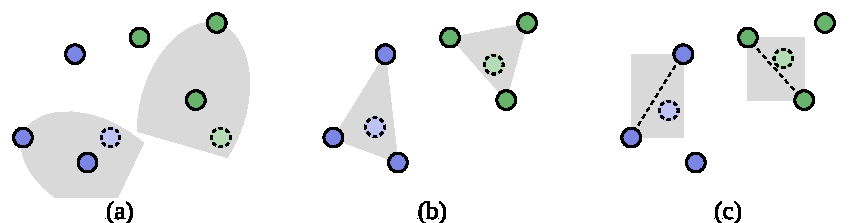
\includegraphics[width=.7\linewidth]{figures/synthetic-data-review/geometric-transformations}
    \caption[Examples of geometric transformation mechanisms.]{%
        Examples of geometric transformation mechanisms. Legend: (a)
        hypersphere mechanism, (b) triangular mechanism and (c)
        hyperrectangle mechanism.
    }~\label{fig:geometric-transformations}
\end{figure}

\subsection{Neural Networks}

Generative Adversarial Network (GAN) architectures are structured as a minimax
two-player game composed of two models, a generator, and a discriminator. Both
models are trained simultaneously throughout the learning phase, to learn to
generate data with similar statistical properties when compared to the
original data. The generative model captures the data distribution, while the
discriminator estimates the probability of an observation coming from the
training data. The goal of the generator model is to produce synthetic
observations that are capable of fooling the discriminator, making it
difficult for the discriminator to distinguish real from synthetic
observations. Although they were originally developed in an unsupervised
learning setting~\cite{goodfellow2020generative}, subsequent contributions
proposed GANs with several different architectures, for semi-SL, supervised
learning (for both regularization and oversampling), and reinforcement
learning.

An autoencoder (AE) is a type of neural network architecture that learns
manifold representations of an input space. These models are typically trained
by regenerating the input and are designed with a bottleneck in the hidden
layers that correspond to the learned latent space. It contains two parts,
an encoder, and a decoder. The encoder transforms the input data into
lower-dimensional representations (\textit{i.e.}, the latent space), while
the decoder projects these representations into the original input space.
Since it was first proposed~\cite{ackley1985learning}, many variants were
developed for multiple applications. However, based on the literature found,
the variational AE architecture appears to be the most popular approach.

